\chapter{Experimental Apparatus}
\label{CHAPTER:ExperimentalApparatus}

\colorbox{red}{
\begin{minipage}{0.95\linewidth}
Should I put anything here?
\end{minipage}
}


\section{The Large Hadron Collider}
\label{SECTION:ExperimentalApparatus_LHC}

\colorbox{red}{
\begin{minipage}{0.95\linewidth}
TODO: 

\begin{itemize}
  \item LHC location, size, particles used, energy usage.
  \item Basics of machine and operation
  \item How instantaneous luminosity is calculated include Instantaneous luminosity equation
  \item Delivered instantaneous luminosity Run I (proton-Proton)
\end{itemize}

\end{minipage}
}

The \gls{LHC} \cite{ARTICLE:LHC Machine} is currently the world's largest particle accelerator and is capable to produce the highest energy particle beam ever made by mankind. This gigantic machine with a total perimeter of 27 kilometer was built at \gls{CERN} in a circular tunnel at an average depth of 100 meters below ground under the Franco-Swiss border near Geneva, Switzerland. I Diagram of the LHC tunnel can be found in figure \ref{FIGURE:ExperimentalApparatus_LHCLayoutUnderground}.

\begin{figure}[!htb]
  \centering
  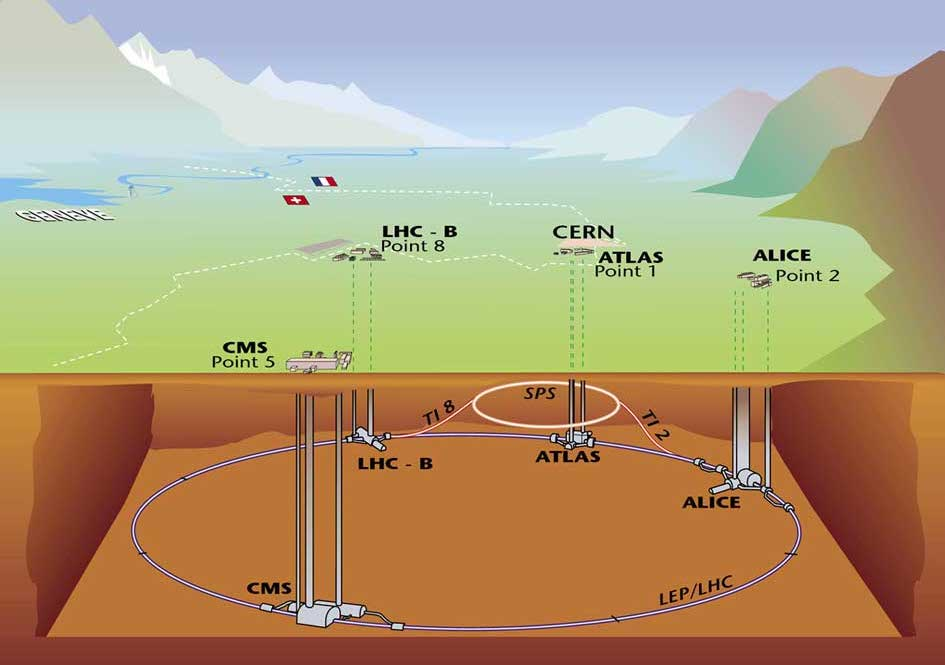
\includegraphics[width=0.50\textwidth]{Chapter02/LHC/Images/LHC_layout_underground.jpg}
  \caption{Underground diagram of the Geneva area showing the \gls{LHC} location.}
  \label{FIGURE:ExperimentalApparatus_LHCLayoutUnderground}
\end{figure}

The \gls{LHC} is a synchrotron machine with the capability to accelerate particles in two separated beam pipes with travel in opposite direction. These beams only cross and are allowed to collide in four specific points of the accelerator where huge particle detectors are installed to detect the products of such collisions. This experiments are name ATLAS, CMS, LHCb and ALICE.

\begin{figure}[!htb]
  \centering
  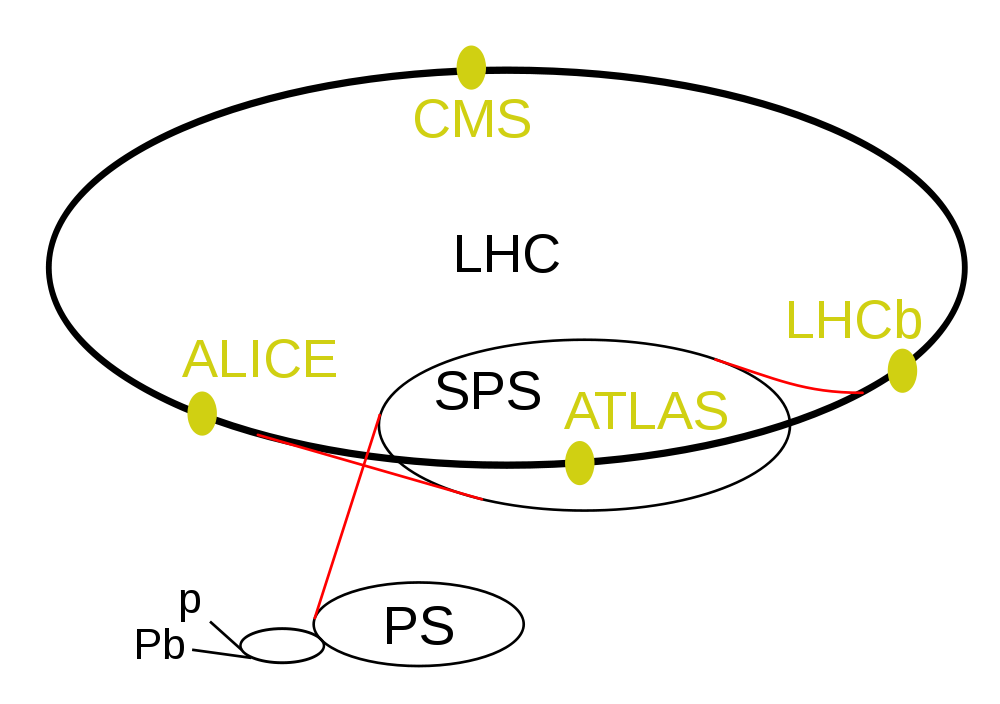
\includegraphics[width=0.50\textwidth]{Chapter02/LHC/Images/LHCAccelaratorChain.png}
  \caption{CERN Large Hadron Collider Experiment accelerator diagram.}
  \label{FIGURE:ExperimentalApparatus_LHCAccelaratorChain}
\end{figure}

The \gls{LHC} is only the last element of a complex accelerator chain which step by step increases the energy of the particles. A simplified diagram of the \gls{CERN} accelerator chain can be found in figure \ref{FIGURE:ExperimentalApparatus_LHCAccelaratorChain}.


\begin{table}[!htb]
  \centering
  \begin{threeparttable}
    \begin{tabular}{|lcccc|}
    \hline 
                                  &              &           \textit{pp} &         \textbf{HI} &  \\
    \hline\hline
    Energy per nucleon            & E            &                     7 &                2.76 &                 $\TeV$ \\
    Dipole field at 7 TeV         & \textit{B}   &                  8.33 &                8.33 &               $\tesla$ \\
    Design Luminosity\tnote{*}    & $\mathcal{L}$ &            $10^{34}$ &           $10^{27}$ & $\cm^{-2}\second^{-1}$ \\
    Bunch separation              &              &                    25 &                 100 &                  $\ns$ \\
    No. of bunches                & $k_B$        &                  2808 &                 592 &                        \\
    No. particles per bunch       & $N_p$        & $1.15 \times 10^{11}$ & $7.0 \times 10^{7}$ &                        \\
    \hline
    \hline
    \textbf{Collisions}           &              &  &  &  \\
    \hline
    $\beta$-value at IP           & $\beta^{*}$  &                  0.55 &                 0.5 &        $\meter$ \\
    RMS beam radius at IP         & $\sigma^{*}$ &                  16.7 &                15.9 &  $\micro\meter$ \\
    Luminosity lifetime           & $\tau_L$     &                    15 &                   6 &         $\hour$ \\
    Number of collisions/crossing & $n_c$        &          $\approx 20$ &                   - &                 \\
    \hline
    \end{tabular}
    \begin{tablenotes}
      \item[*] For heavy-ion (HI) operation the design luminosity for Pb-Pb collisions is given.
    \end{tablenotes}
  \end{threeparttable}
  \caption[LHC parameters relevant for detectors]{The machine parameters relevant for the 
                                                  LHC detectors.\cite{CMSTDR:CMSPhysicsVol1}}
  \label{TABLE:ExperimentalApparatus_LHCMachineParameters}
\end{table}


%
% The Large Hadron Collider (LHC) is at this moment the world's largest and highest-energy particle accelerator
% in activity. I was built in a 27 kilometer circular tunnel, at a average depth of around 100 meters under the
% Franco-Swiss border near Geneva, Switzerland.
% 
% The LHC a synchrotron machine designed to collide two opposing particle beams of protons each one with a 
% maximum energy of 7 TeV per proton and for lead nuclei beams a maximum of 574 TeV per nucleus. Providing a 
% maximum available energy of 14 TeV in the center of mass frame for a single proton-proton.
% 
% To be able to accelerate protons (and ions) to such high energies the LHC relies on a chain of other accelerator
% machines (fig. \ref{ExperimentalApparatus_LHCAccelaratorChain}). For protons, it all starts at the Linear 
% Particle Accelerator 2 (LINAC2) which get protons to 50 MeV, they are injected into the Proton Synchrotron
% Booster (PSB) which further accelerates them to 26 GeV. After getting to this energy, protons go into the Super 
% Proton Synchrotron (SPS) where the get accelerated to 450 GeV. When maximum energy at SPS is reached protons
% can get injected into the LHC in bunches, where they finally get accelerated to the maximum energy of 7 TeV. 
% A single fill of proton bunches can be circulated and collided maintaining rates of collisions from 10 to 24 hours. 



Luminosity Equation

\begin{equation}
L=\frac{N_{b}^{2}n_{b}f_{\text{rev}}\gamma}{4\pi\epsilon_{n}\beta^{*}}F,
\end{equation}

\section{The Compact Muon Solenoid Experiment}
\label{SECTION:ExperimentalApparatus_CMS}

The \gls{CMS} experiment is located at point 5 of the \gls{LHC}.





\subsection{Tracker}
\label{SUBSECTION:ExperimentalApparatus_CMS_Tracker}

\subsection{Electromagnetic Calorimeter}
\label{SUBSECTION:ExperimentalApparatus_CMS_ECAL}

The \gls{ECAL} 


\subsection{Hadronic Calorimeter}
\label{SUBSECTION:ExperimentalApparatus_CMS_HCAL}

The \gls{HCAL}

\subsection{Solenoid Magnet}
\label{SUBSECTION:ExperimentalApparatus_CMS_Magnet}

\begin{table}[!htb]
  \centering
  \begin{tabular}{|l|c|}
  \hline
  Parameter & Value \\
  \hline\hline
  Field           & 4 T \\
  Inner Bore      & 5.9 m \\
  Length          & 12.9 m \\
  Number of turns & 2168 \\
  Current         & 19.5 kA \\
  Stored Energy   & 2.7 GJ \\
  Hoop Stress     & 64 atm \\
  \hline
  \end{tabular}
  \caption[Parameters of the CMS superconducting solenoid]{Parameters of the CMS superconducting solenoid}
  \label{TABLE:ExperimentalApparatus_CMSMagnetParameters}
\end{table}


\subsection{Muon System}
\label{SUBSECTION:ExperimentalApparatus_CMS_Mouns}

\subsection{Data Acquisition System}
\label{SUBSECTION:ExperimentalApparatus_CMS_DAQ}

The \gls{DAQ}

\subsection{Trigger System}
\label{SUBSECTION:ExperimentalApparatus_CMS_Trigger}

The \gls{L1T} and \gls{HLT}

\subsection{Computing}
\label{SUBSECTION:ExperimentalApparatus_CMS_Computing}

The \gls{DQM} 

\subsection{Run II Updgrades}
\label{SUBSECTION:ExperimentalApparatus_CMS_RUNII}

The upgrade tdr \cite{CMSTDR:CMSL1Upgrade}.
